% Options for packages loaded elsewhere
\PassOptionsToPackage{unicode}{hyperref}
\PassOptionsToPackage{hyphens}{url}
%
\documentclass[
]{book}
\usepackage{amsmath,amssymb}
\usepackage{lmodern}
\usepackage{iftex}
\ifPDFTeX
  \usepackage[T1]{fontenc}
  \usepackage[utf8]{inputenc}
  \usepackage{textcomp} % provide euro and other symbols
\else % if luatex or xetex
  \usepackage{unicode-math}
  \defaultfontfeatures{Scale=MatchLowercase}
  \defaultfontfeatures[\rmfamily]{Ligatures=TeX,Scale=1}
\fi
% Use upquote if available, for straight quotes in verbatim environments
\IfFileExists{upquote.sty}{\usepackage{upquote}}{}
\IfFileExists{microtype.sty}{% use microtype if available
  \usepackage[]{microtype}
  \UseMicrotypeSet[protrusion]{basicmath} % disable protrusion for tt fonts
}{}
\makeatletter
\@ifundefined{KOMAClassName}{% if non-KOMA class
  \IfFileExists{parskip.sty}{%
    \usepackage{parskip}
  }{% else
    \setlength{\parindent}{0pt}
    \setlength{\parskip}{6pt plus 2pt minus 1pt}}
}{% if KOMA class
  \KOMAoptions{parskip=half}}
\makeatother
\usepackage{xcolor}
\usepackage{longtable,booktabs,array}
\usepackage{calc} % for calculating minipage widths
% Correct order of tables after \paragraph or \subparagraph
\usepackage{etoolbox}
\makeatletter
\patchcmd\longtable{\par}{\if@noskipsec\mbox{}\fi\par}{}{}
\makeatother
% Allow footnotes in longtable head/foot
\IfFileExists{footnotehyper.sty}{\usepackage{footnotehyper}}{\usepackage{footnote}}
\makesavenoteenv{longtable}
\usepackage{graphicx}
\makeatletter
\def\maxwidth{\ifdim\Gin@nat@width>\linewidth\linewidth\else\Gin@nat@width\fi}
\def\maxheight{\ifdim\Gin@nat@height>\textheight\textheight\else\Gin@nat@height\fi}
\makeatother
% Scale images if necessary, so that they will not overflow the page
% margins by default, and it is still possible to overwrite the defaults
% using explicit options in \includegraphics[width, height, ...]{}
\setkeys{Gin}{width=\maxwidth,height=\maxheight,keepaspectratio}
% Set default figure placement to htbp
\makeatletter
\def\fps@figure{htbp}
\makeatother
\setlength{\emergencystretch}{3em} % prevent overfull lines
\providecommand{\tightlist}{%
  \setlength{\itemsep}{0pt}\setlength{\parskip}{0pt}}
\setcounter{secnumdepth}{5}
\usepackage{booktabs}
\ifLuaTeX
  \usepackage{selnolig}  % disable illegal ligatures
\fi
\usepackage[]{natbib}
\bibliographystyle{apalike}
\IfFileExists{bookmark.sty}{\usepackage{bookmark}}{\usepackage{hyperref}}
\IfFileExists{xurl.sty}{\usepackage{xurl}}{} % add URL line breaks if available
\urlstyle{same} % disable monospaced font for URLs
\hypersetup{
  pdftitle={Conservation Decisions Lab Handbook},
  pdfauthor={Conservation Decisions Lab},
  hidelinks,
  pdfcreator={LaTeX via pandoc}}

\title{Conservation Decisions Lab Handbook}
\author{Conservation Decisions Lab}
\date{2024-02-20}

\begin{document}
\maketitle

{
\setcounter{tocdepth}{1}
\tableofcontents
}
\begin{center}\rule{0.5\linewidth}{0.5pt}\end{center}

\hypertarget{overview}{%
\chapter*{Overview}\label{overview}}
\addcontentsline{toc}{chapter}{Overview}

\begin{center}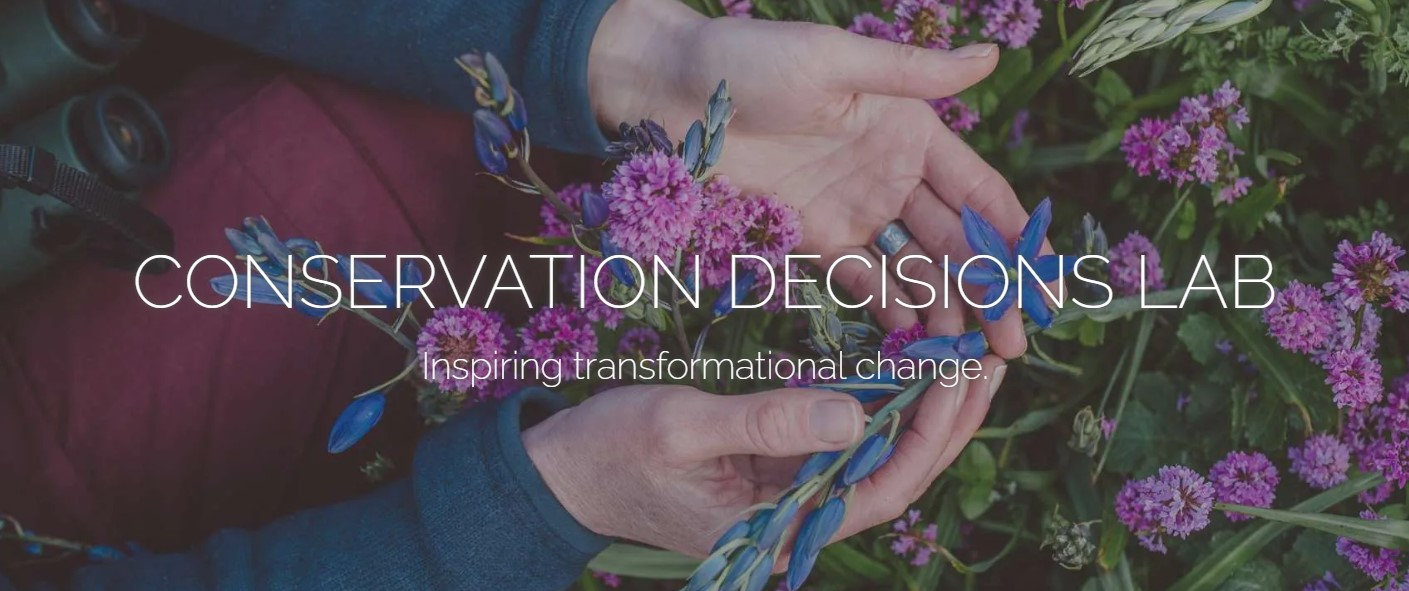
\includegraphics[width=0.5\linewidth]{img/cdl-lab-banner} \end{center}

This document is a brief introduction to the Conservation Decisions Lab. It provides:

\begin{itemize}
\item
  Insight into \protect\hyperlink{diversity}{lab values} and \protect\hyperlink{expectations}{expectations}
\item
  Need to know details about your \protect\hyperlink{computers}{workstation}
\item
  Information about \protect\hyperlink{safety}{safety} in the lab and in the field
\item
  Common practices for \protect\hyperlink{working}{working in the lab and from home}
\item
  The \protect\hyperlink{social}{social} atmosphere in the lab
\item
  The lab \protect\hyperlink{vehicle}{vehicle} and when/how it can be used
\item
  All things related to your \protect\hyperlink{thesis}{thesis} and how to get ahead of the curve
\item
  \protect\hyperlink{resources}{Resources} for anyone new to UBC or Vancouver
\end{itemize}

\hypertarget{welcome}{%
\chapter*{Welcome}\label{welcome}}
\addcontentsline{toc}{chapter}{Welcome}

Welcome to the \href{https://www.taramartin.org/}{Conservation Decisions lab} (CDLab) where your supervisor, Dr.~Tara Martin aspires to inspire innovation, excellence in critical thinking, excellent quantitative skills and the ability to think and work across disciplines as conservation practitioners.

This student handbook has been designed as a guide to assist your transition into the UBC community and the community of the Conservation Decisions Lab. Within its contents you will find tips, tricks, and essential information for you as a student and as a lab member.

If you find any information missing from the following pages or have any recommendations that could improve this guide please contact the CDLab manager, Abbie Sherwood who strives to make this an exhaustive resource.

Please read this document in its entirety early on within your appointment to ensure that as a new lab member you are aware of the resources at your disposal and what is expected of each and every lab member. Dr.~Tara Martin has committed to creating an active community within her lab space where she encourages the development of good collaborators and lab citizens. Within this space we commit to being intelligent, curious, motivated, compassionate, and hard-working.

Thank you for joining us in our efforts to turn ecological data into decision making

\hypertarget{diversity}{%
\chapter*{Equity Diversity and Inclusion Policy}\label{diversity}}
\addcontentsline{toc}{chapter}{Equity Diversity and Inclusion Policy}

To begin we would like to introduce \href{https://www.taramartin.org/equity-diversity-and-inclusion/}{our equity, diversity and inclusion (EDI) policy}. The Martin Conservation Decisions Lab (CDL) and the Arcese Lab at the University of British Columbia---led by Dr.~Tara Martin and Dr.~Peter Arcese, respectively---have worked together to develop this Equity, Diversity, and Inclusion (EDI) Statement. We recognize the colonial contexts of conservation and academia, both past and present, and the systemic inequities that prevail. We see it as our responsibility to encourage, include, and make way for underrepresented and marginalized voices and perspectives, meaningfully collaborate with and support the work of Indigenous communities, and to communicate our research to a broad cross-section of society across all demographics. We strive to decolonize the science that we do from the questions we pose, to the manner in which we undertake and communicate the science.

Our labs are committed to recruiting and collaborating with people of diverse backgrounds, identities, experiences, and perspectives. We believe that diversity is critical for transforming us into better students, teachers, scientists, conservation practitioners, and members of our communities. The challenges we face in conservation and as a society at large---whether they be related to biodiversity, climate change, and/or EDI---require a shared understanding, novel perspectives, and transformative actions. We are actively working to reduce barriers to diverse representation in our research, in conservation, and in academia. Through this process, we aim to share knowledge, experience, and insight with each other that can be applied to our future workplaces, many of which share similar legacies of systemic inequality.

We acknowledge that our labs---centred at UBC Vancouver---are located on the traditional, ancestral, and unceded territory of the Coast Salish people.\href{https://indigenous.ubc.ca/indigenous-engagement/musqueam-and-ubc/}{The land where UBC is situated has always been a place of learning where people for millennia have passed on their culture, history, and traditions from one generation to the next on this site.} Members of our lab engage in research on this land, as well as in the territories of other First Nations in BC and Indigenous communities across Canada and the world. We have a duty to reflect and reconcile the nature of our work with the history and ongoing nature of colonialism, academic research, and Indigenous dispossession. It is our intent to foster meaningful relationships with the communities whose lands we are working on and engage in a research process that is beneficial to and is anchored by the values, goals, and interests of those communities.

We acknowledge that each of us may be at different points throughout our journey in learning, listening, and cultivating an inclusive academic environment and that mistakes can be made. We also understand how important it is to learn from those mistakes and to not let the fear of making a mistake be an excuse for inaction. To guide our journey, we are committed to continuously revisiting these values and updating this EDI statement as a living document.

We welcome feedback and inquiries concerning this statement. If you are a prospective student or collaborator and would like to know more about our lab policies, please reach out to the CDLab manager with any comments, or to discuss any aspect of EDI related to our labs.

\hypertarget{values}{%
\section*{Our Values}\label{values}}
\addcontentsline{toc}{section}{Our Values}

We value diversity of identities, knowledge systems, and worldviews in our lab and community.

We value a lab culture whereby we can reflect on our personal and collective identities, both as researchers and as colleagues. This means we are actively acknowledging the intersecting privilege and/or barriers that we may or may not face associated with our identities.

We value acceptance. Discrimination---e.g., unjust treatment on the basis of sex, race, gender identity, sexual orientation, religion, socioeconomic background, national origin, education level, physical and mental ability, age, physical appearance, political views---in any form will not be tolerated within this space. Derogatory or hurtful comments will not be accepted and all lab members are encouraged to initiate discussion when inappropriate behavior or language is observed.

We value accountability in supporting and nurturing a culture of safety within our team. All members of our team commit to creating a safe, supportive, respectful, and inviting community.

We value an ongoing and iterative journey of learning. We recognize the continuous commitment of (un)learning necessary to build a more equitable, diverse, and inclusive community.

\hypertarget{ediactions}{%
\section*{Actions}\label{ediactions}}
\addcontentsline{toc}{section}{Actions}

\hypertarget{individualactions}{%
\subsection*{Individual Actions}\label{individualactions}}
\addcontentsline{toc}{subsection}{Individual Actions}

\begin{itemize}
\tightlist
\item
  Be prepared to examine one's own bias and privilege
\item
  Devote time to continue learning about EDI issues, working through provided EDI materials, sourcing new materials and contributing to the lab's EDI materials library.
\item
  Practice deep listening to ensure we are working with peers and collaborators in a meaningful way, rather than dictating or projecting our needs onto others.
\item
  Welcome critiques of our words and actions, and remain open to engaging in uncomfortable conversations that are integral to change. Complete UBC's conflict engagement course here
\item
  Invite speakers, panels, authorship, and committees to better represent the diversity of perspectives and lived experiences.
\item
  Use any privilege (eg. status or experience) to provide space for underrepresented or overlooked contributors before ourselves.
\item
  Consider including local knowledge holders, practitioners, and scientists from other disciplines in our research during study design, questions, analyses, and writing.
\item
  Communicate and provide research outputs to those involved and affected by the research and possible decisions influenced by this research.
\item
  Commit to open science and data sharing when appropriate (e.g., with the permission of any data that might be sensitive).
\item
  Question and adapt methods to be more open to other forms of knowledge.
\item
  Use inclusive pronouns and language.
\item
  Be willing to share ideas, projects, and concepts with others.
\end{itemize}

\hypertarget{labactions}{%
\subsection*{Lab Community Actions}\label{labactions}}
\addcontentsline{toc}{subsection}{Lab Community Actions}

\begin{itemize}
\tightlist
\item
  Use this document as a social contract to foster a safe space within our lab community.
\item
  Actively update this document to reflect new perspectives and growth annually during lab events.
\item
  Devote time to discussing EDI materials, including EDI focused activities and group exercises during lab events.
\item
  Provide resources for members to attend EDI courses, training, and workshops.
\item
  Continuously build and update the online and physical EDI learning library in the lab.
\item
  Invite speakers, panels, authorship, and committees to better represent diversity of perspectives and lived experiences.
\item
  Facilitate discussion aimed to educate and encourage lab members on the best practices of including local knowledge holders, community groups, practitioners, and scientists from other disciplines in our research.
\item
  Ensure that lab events are inclusive, accessible and safe for all lab members by providing multiple event options for venues and activities.
\end{itemize}

\hypertarget{researchpractices}{%
\section*{Best Practices in Research}\label{researchpractices}}
\addcontentsline{toc}{section}{Best Practices in Research}

We are committed to building our fluency and capacity in the following areas to facilitate best practices in EDI in our research:

\begin{itemize}
\item
  Acknowledging power and vulnerabilities

  \begin{itemize}
  \tightlist
  \item
    Follow best practices in EDI in hiring and retainment, and encourage the department (Biodiversity Cluster?) to follow suite
  \item
    Encourage reflexivity and positionality statements in grad student/postdoc applications
  \item
    Provide basic EDI training when involved in a hiring process
  \item
    Participate in basic EDI training when involved in a hiring process
  \item
    confronting harassment in the workplace
  \end{itemize}
\item
  Committing to transparency and accountability to the implications of our works
\item
  E.g., who benefits, who is impacted?
\item
  Titleholder and stakeholder engagement throughout the research process
\item
  Clarity around ownership and control of data
\item
  Fairly acknowledging contributions
\item
  Encourage reflexivity and positionality statements in your work and research
\item
  Committing to accessibility
\item
  E.g., Communicating our research to diverse audiences
\item
  Open access data (where appropriate), code, and publications
\item
  Examining reward systems within and beyond academia (e.g., what constitutes ``good'' research questions, reward systems for research participants)
\item
  Equitable hiring relative to opportunities (e.g., consider paid positions vs volunteers, make space early and often for conversations around additional resources and capacity for hiring graduate students and PDFs)
\item
  Decolonizing our approach to research
\item
  E.g., Fostering collaborative approaches to co-developing research, practicing accountability (e.g., ``helicopter research''), and being open to timeframes and reward systems outside of academia
\item
  Access training for appropriate ethics (e.g., UBC and Nation/community-specific intake processes), communication, and decolonizing
\item
  ``Doing our homework'' - knowing where we work and the historical context of the systems we get to work in
\item
  Be open and curious to multiple ways of knowing, learning, and communicating
\item
  Daylighting health and wellness
\item
  Prioritizing our own and each other's mental health in grad school
\item
  Openly discussing / holding space for health and wellness obstacles, personally and professionally (i.e., in academic spaces)
\item
  Celebrating success beyond the h-index and the awards list!
\end{itemize}

\hypertarget{ediresources}{%
\section*{Resources}\label{ediresources}}
\addcontentsline{toc}{section}{Resources}

As a part of our EDI commitment we have established an \href{https://docs.google.com/document/d/102fsqZL8UVf22TX1kTZ1WjQu2U9SrFjEBbQ9NipedXA/edit\#heading=h.axugsem4agey}{online resources center} for EDI related materials. This is by no means a complete or exhaustive list. We encourage all lab members to add to this resource pool. Thank you in advance for contributing material that you believe will assist in our collective education.

\hypertarget{lab-member-commitments}{%
\chapter{Lab Member Commitments}\label{lab-member-commitments}}

\hypertarget{lab-meetings}{%
\section{Lab Meetings}\label{lab-meetings}}

All lab members are expected to attend our lab meetings which take place every three weeks. Meetings are held in our lab room and off campus students are able to join virtually. When the lab meetings are hosted at UBC, it is expected that all lab members are to attend face-to-face in order ensure that all lab members have the opportunity to socialize with other members, however we understand that exceptions must be made due to circumstance.

When meetings are scheduled while under a public health order or regulation these meetings will be held virtually via Zoom.

Lab meetings present an opportunity for lab members to showcase their current work or work that they have done in the past and practice for upcoming presentations or thesis defense. These meetings also serve as a platform that provides space for members to bring any topic to the table for discussion. Each lab member is expected to lead a lab meeting twice a year. The sign-up sheet for the lab meeting facilitators can be found \href{https://docs.google.com/spreadsheets/d/1WAL131F2qjLT-kYOPUGV7lpESvUIczRtx1Q2oqTfdRQ/edit\#gid=740242269}{here} along with historical lab meeting topics.

The lab meetings will be scheduled with every new semester and will be timed according to the collective availability of the lab community. Once determined the lab meeting schedule will be sent out to all lab member by the CDLab manager who will also send out meeting reminders and any related material that are to be reviewed prior to the lab meeting.

As part of the commitment that our lab community has made in our EDI statement these lab meetings will commonly be used as a time and platform for EDI related conversations. This is a safe and confidential space where lab members are welcome to ask hard questions, be met with compassionate and difficult answers and to explore new and deeper components of our own experience through conversation within community. Please remember that during these difficult and vital conversations you are not expected to adhere your boundaries to anyone else's but that if you are comfortable to expand your comfort zone this is an excellent and safe space with which to do so.

\hypertarget{on-1-meetings}{%
\section{1-on-1 Meetings}\label{on-1-meetings}}

Mentees will meet with Dr.~Tara Martin for a 1-on-1 meeting every three weeks. The default length of these meetings are 30 minutes although an extended meeting is available upon request. The CDLab manager will schedule these meetings at the beginning of each semester and will send out event invites and zoom links when meetings will be held virtually and in person. Please direct any scheduling questions to the CDLab manager.

\hypertarget{newvancouver}{%
\chapter*{New to Vancouver}\label{newvancouver}}
\addcontentsline{toc}{chapter}{New to Vancouver}

This is by no means an exhaustive list of tips and tricks for those who are new to the great city of Vancouver. Many of our lab members are from elsewhere in Canada and the world and so have gone through the process of moving and settling in Vancouver, and will be happy to give tips. We urge for you to communicate via our \protect\hyperlink{slack}{slack}, via email or in person with other lab members who live in Vancouver and who will be able to provide more information and suggestions on how to enjoy the city to it's fullest extent.

\hypertarget{vancouverculture}{%
\section*{Cultural Awareness}\label{vancouverculture}}
\addcontentsline{toc}{section}{Cultural Awareness}

As stated in our lab's EDI statement Dr.~Tara Martin encourages and supports lab members to take time to become aware of the culture surrounding Vancouver and the areas where research is conducted and beyond.

It is expected that each lab member begins to familiarize themselves with the lush cultural surroundings of Vancouver and the Point Grey Campus. You will notice that a land acknowledgment is common practice during introductions. UBC provides \href{https://guides.library.ubc.ca/distance-research-xwi7xwa/landacknowledgements}{a guide} to assist those new to the land acknowledgment practice and we encourage all lab members to participate in this brief yet vital `Respect, Sincerity \& Responsibility: Land Acknowledgements @ UBC' course. Enroll \href{https://wpl.ubc.ca/browse/orientation-and-onboarding/courses/wpl-oo-ilpla}{here}.

For those incoming lab members that are new to Canada and Canadians alike, we highly recommend and encourage enrolling in the `\href{https://www.coursera.org/learn/indigenous-canada}{Indigenous Canada}' course offered by the University of Alberta and hosted by coursera which provides effective context to Canada's history of colonization. This is a great course and is expected to take 21 hours to complete.

We also greatly encourage new lab members to familiarize themselves with the \href{https://indigenous.ubc.ca/longhouse/fnhl/}{First Nations House of Learning} at UBC which is an incredible resource and provides opportunity to learn about how you can actively work to decolonize your own world view.

\hypertarget{vancouverevents}{%
\section*{Events}\label{vancouverevents}}
\addcontentsline{toc}{section}{Events}

There are many \href{https://www.destinationvancouver.com/events/calendar-of-events/}{festivals and events throughout the year in Vancouver}. Some that are recommended by lab members are:
* Cherry Blossom Festival (April)
* Celebration of Light (July)
* Vancouver Folk Music Festival (July)
* Pride (BC Day weekend, August)
* Vancouver International Film Festival (September)
* Fringe Festival (September)
* Westward Music festival (September)
* Vancouver Christmas Market (November-December)

\hypertarget{statutory-holidays--statutory}{%
\section{Statutory Holidays \{-\$statutory\}}\label{statutory-holidays--statutory}}

Statutory holidays recognized as paid holidays by UBC can be found listed \href{https://hr.ubc.ca/working-ubc/statutory-holidays}{here}.

\hypertarget{housing}{%
\section*{Housing}\label{housing}}
\addcontentsline{toc}{section}{Housing}

There are 14 on-campus residences at UBC Vancouver. Visit \url{https://vancouver.housing.ubc.ca/} to find out more.

If you are planning a move to Vancouver some of the most effective resources are Facebook, Craigslist, and Used Vancouver. Some have also had success by walking the neighborhoods they are interested in looking for vacancy signs out the front of buildings.

There are many Facebook groups that advertise rentals, sublets and housemates, including Vancouver Rentals and Roommates, For Rent Vancouver, Vancouver apartments/houses for rent/roommates, Vancouver Buy/Sell Fast and Aussies in Vancouver. We encourage the use of our \protect\hyperlink{slack}{Slack} where new members may ask housing related questions of those how have also gone through the process of finding housing in Vancouver.

It is worth knowing that in BC, lease periods begin on the 1st of the month and sometimes on the 15th. The term of lease agreement varies from month to month, three months, 6 months, and a year.

For those who are new to renting the \href{https://www2.gov.bc.ca/gov/content/housing-tenancy}{Housing and tenancy page of the BC government website} provides great resources on how to ensure that you legally protect yourselves as a tenant. It is highly recommended to ensure that your landlord provides you with a \href{https://www2.gov.bc.ca/gov/content/housing-tenancy/residential-tenancies/starting-a-tenancy/tenancy-agreements}{lease agreement} regardless of history or personal connections.

\hypertarget{newtoubc}{%
\chapter*{New to UBC}\label{newtoubc}}
\addcontentsline{toc}{chapter}{New to UBC}

We recommend that all graduate students keep the \href{https://forestry.ubc.ca/files/2023/04/Forestry-Gradbook.pdf}{GRADBOOK} close at hand. This document outlines the policies and procedures for Forestry graduate students.

Here is a link to the \href{https://forestry.ubc.ca/students/graduate-student-portal/}{graduate student portal} where you will find links to \href{https://forestry.ubc.ca/students/graduate-student-portal/graduate-student-advising/}{graduate studies advising} and links to \href{https://forestry.ubc.ca/students/graduate-student-portal/financial-support/}{financial support opportunities} among many other resources.

\hypertarget{forestrybuildinglocale}{%
\section*{Foresty Building Location}\label{forestrybuildinglocale}}
\addcontentsline{toc}{section}{Foresty Building Location}

You can use the \href{https://www.maps.ubc.ca/}{UBC wayfinder} to locate rooms and buildings on campus.

Mailing address:
Forestry and Conservation Sciences (FCS)
3041-2424 Main Mall
Vancouver
B.C. V6T 1Z4

\hypertarget{building-access}{%
\section{Building Access}\label{building-access}}

Access to individual offices requires a key, which will be requested by FCS reception and issued by the Access Desk at the Bookstore, with a \$20 security deposit (this information is from the 2020 academic year). Most students will not be provided with an office but will use the lab space as work stations.

Since 2020, the FCS building has undergone a change of key system. As September 2021 approaches all lab members will receive an updated email from the FCS reception desk and the CDLab manager regarding new access processes which will utilize student/employee key cards.

For card configuration issues see \protect\hyperlink{contacts}{Andrea Chan}.

For after hours access issues call Campus Security 604 822 2222.

\hypertarget{labroom}{%
\section*{Lab Room}\label{labroom}}
\addcontentsline{toc}{section}{Lab Room}

Our lab room 3202 and includes the kitchen facilities, lounge, desks and conference table. Please be considerate of anyone using the desks in the lab room.

The main meeting rooms used by the lab are rooms 3003 and 3101 (known as `The Fishbowl'). Room 3003 includes a TV and webcam that can be connected to a laptop via HDMI. Room 3101 has wall space for a projector, which can be borrowed from FCS Reception (try to book in advance). These rooms must be booked in advance through \protect\hyperlink{contacts}{Natasha Thompson} at the FCS reception, and a key obtained from her at time of use.

\hypertarget{commonspaces}{%
\section*{Common Spaces}\label{commonspaces}}
\addcontentsline{toc}{section}{Common Spaces}

The kitchen on level 3 is room 3039. This is available to all staff, students and faculty, but is closed at 4:30 each day. There is a kitchen and dining area on level 4 (room 4003) that is for staff and faculty use only, unless it is booked for an event.

Desks and lounge areas include the level 3 landing, and the Treehouse, which is the study space in the atrium with all the plants.

\hypertarget{printing}{%
\section*{Printing/Copying}\label{printing}}
\addcontentsline{toc}{section}{Printing/Copying}

Room 3005 is the copy room for FCS. The photocopy code assigned to Tara and the lab is 426520, which is charged to Tara's start-up fund.

\hypertarget{ubcsocial}{%
\section*{UBC Social Events}\label{ubcsocial}}
\addcontentsline{toc}{section}{UBC Social Events}

\hypertarget{seminars}{%
\subsection{Seminars}\label{seminars}}

There are regular seminars held during the school year by the Department and open to staff, students and faculty. These include the \href{https://zoology.ubc.ca/events/weekly-seminars/friday-comparative-physiology-invited-speaker-seminar}{Comparative Physiology seminar series} and the FCS Wednesday seminar series. Notification of the FCS seminar is emailed to all staff, faculty and grad students. To be notified of other seminars and discussions, join email lists (see section 2.1.2).

\hypertarget{biodiversity-beers}{%
\subsection{Biodiversity Beers}\label{biodiversity-beers}}

Biodiversity Beers is a social event held in the atrium of the Biodiversity Building every Friday at 5pm. All are welcome to attend, and also to \href{https://blogs.ubc.ca/biodiversitysocial/volunteer-information/}{volunteer for the buying/serving of drinks}.

Notifications for the event come through the zoology \protect\hyperlink{emaillists}{email list}.

\hypertarget{hazardous-waste}{%
\section{Hazardous Waste}\label{hazardous-waste}}

Information about hazardous waste disposal at UBC can be found \href{https://srs.ubc.ca/environment/hazardous-waste-management/hazardous-waste-manual/}{here}.

Some items/substances that may be used in the lab and are subject to safe disposal protocols are:
* Sharps (syringes, razors, blades)
* Animal blood
* Uncontaminated animal carcasses
* Non-indigenous species (includes soil and plants)

Disposal of biological waste may require special training. Contact Rolando Descalzo, Collections Manager, for waste disposal inquires (\href{mailto:rolando.descalzo@ubc.ca}{\nolinkurl{rolando.descalzo@ubc.ca}}).

Sharps disposal containers can be purchased from the Chemistry Store on the corner of Main Mall and University Boulevard using a journal voucher.

\hypertarget{transportation}{%
\chapter*{Getting to UBC}\label{transportation}}
\addcontentsline{toc}{chapter}{Getting to UBC}

\hypertarget{bus}{%
\section{Bus}\label{bus}}

Buses that run between downtown and UBC include the 44, 4 and 14. The 99 B-line service also terminates at UBC. Many buses will take you to nearby Skytrain stations, such as VCC-Clark and Bridgeport.

The information about U-Pass BC/Compass card which provides UBC students with universal, accessible and affordable access to public transit across the Metro Vancouver Region can be found \href{https://planning.ubc.ca/transportation/transit/u-pass-compass-card}{here}. UBC students pay for this pass via the mandatory student fees collected by UBC.

A Compass card is the most cost-effective way of using Skytrains and buses, although cash and credit card are also accepted at tap-on points. Compass cards can be purchased at vending machines in Skytrain stations, UBC Bookstore, ferry terminals, and some London Drugs, Save on Foods and 7eleven outlets. For UBC students, the U-Pass can be added to your Compass card to give unlimited access to Skytrain, Canada Line and SeaBus services.

A useful public transport app is `Transit', which can be downloaded for free. Transport options include Skytrain, buses, bike share (Shaw bikes in the downtown area, or Hopr bikes on campus), and car share (Evo, Modo).

\hypertarget{car}{%
\section{Car}\label{car}}

Car parking is available next to Forestry on Agronomy Road (\$20/day). Parking permits can be purchased \href{https://parking.ubc.ca/permits-rates}{here}. Designated parking stalls are available for car share services.

Uber or Lyft are ride sharing apps that can be used as an alternative.

\hypertarget{bike}{%
\section{Bike}\label{bike}}

Public bike racks are available outside of the FSC building. Unfortunately bicycle theft is a problem in Vancouver and at UBC so please keep your bike safe with a lock. The FSC complex also has secured bike racks in room 0711 in the basement. Space is limited, inquire at FCS Reception.

\hypertarget{from-vancouver-island}{%
\section{From Vancouver Island}\label{from-vancouver-island}}

The 480 bus to Bridgeport station will link up with buses that go to Tsawwassen Ferry Terminal. Buses 44, 4 and 14 stop at Waterfront Station, linking up with buses that go to Horseshoe Bay Ferry Terminal. The seaplane terminal is also a short walk from Waterfront Station.

\hypertarget{contacts}{%
\chapter*{Useful Contacts}\label{contacts}}
\addcontentsline{toc}{chapter}{Useful Contacts}

A contact list for all lab members (including the Arcese lab), contacts within the university, and external project-related contacts can be found on the \protect\hyperlink{sharednetworkdrive}{shared Z drive} and on the \protect\hyperlink{dropbox}{shared Dropbox folder}. There are many UBC employees that are equipped with knowledge that can make the transition from a new student to an informed student seamless.

Contacting the current CDLab manager with inquiries is always welcome and encouraged. Please do not hesitate to ask for guidance in regards to whom to contact with questions or concerns.

Natasha Thompson (\href{mailto:Natasha.thompson@ubc.ca}{\nolinkurl{Natasha.thompson@ubc.ca}}) is the FCS receptionist -- is the go-to person for general admin related to the department.

Andrea Chan (\href{mailto:andrea.chan@ubc.ca}{\nolinkurl{andrea.chan@ubc.ca}}) is an FCS administrator -- Salary, training, hiring paperwork, taxes, graduate research assistant hiring.

Christine Mutia (\href{mailto:christine.mutia@ubc.ca}{\nolinkurl{christine.mutia@ubc.ca}}) is our Finance Specialist for FSC -- out of pocket expenses.

Rosemarie Cheng (\href{mailto:rosemarie.cheng@ubc.ca}{\nolinkurl{rosemarie.cheng@ubc.ca}}) -- grant management Alice Miao (\href{mailto:alice.miao@ubc.ca}{\nolinkurl{alice.miao@ubc.ca}}) -- Grant application, NSERC, application and processing of grants.

Norm Hodges -- IT (\href{mailto:norman.hodges@ubc.ca}{\nolinkurl{norman.hodges@ubc.ca}})

\hypertarget{ubconlineaccess}{%
\chapter*{UBC Online Access}\label{ubconlineaccess}}
\addcontentsline{toc}{chapter}{UBC Online Access}

Once you have received your student number and your first-time sign in information visit The \href{https://activate.id.ubc.ca/iamweb/}{University of British Columbia} to establish your UBC Campus Wide Login (CWL). This CWL is your one place sign in for all of the UBC portals that will be at your disposal.

The CDLab manager will send IT (Norm Hodges) and email requesting that you obtain access to the Forestry drives of UBC. They will Cc you in this email as your CWL will be required.

The Forestry drives of UBC will give you access to secure data storage spaces and access to the shared lab Z drive. \href{https://it.ubc.ca/services/web-servers-storage/home-drive-storage-service/mapping-or-mounting-your-home-drive-0}{Here is a link} to how you can map to this shared drive space.

Be aware that some UBC software, like ArcGIS, only functions when using the UBC VPN -- Cisco AnyConnect Secure Mobility Client. \href{https://it.ubc.ca/services/email-voice-internet/myvpn/setup-documents}{Here is a guide} as to how to set up your VPN for remote access away from the UBC campus.

For more information on how to access the IT services of UBC (see section 2.1)

\hypertarget{orientation}{%
\chapter*{New Student Orientation}\label{orientation}}
\addcontentsline{toc}{chapter}{New Student Orientation}

There are multiple orientation sessions that new graduate students can attend. We would like to recommend attending them all as each provides new students with great information and highlights the UBC resources available to you during you time as a student at UBC.

Using your CWL information log into your UBC instructure account \url{https://ubc.instructure.com/} where you will be able to enroll in an assortment of \href{https://wpl.ubc.ca/}{courses}:

\begin{enumerate}
\def\labelenumi{\arabic{enumi})}
\tightlist
\item
  New student orientation This orientation power point can also be found in the Conservation decisions Lab dropbox folder here.
\item
  Forestry Graduate Programs Canvas Course This link directs you to the Forestry Graduate Program Hub where you can connect with your peers and colleagues across departments; share and receive wellness and organizational tips; join and participate in stress-lowering online activities and events; and, network with others in multiple ways as we all move through the pandemic together.
\end{enumerate}

\hypertarget{workplacetraining}{%
\section*{Workplace Training}\label{workplacetraining}}
\addcontentsline{toc}{section}{Workplace Training}

There are a number of mandatory online training modules staff and students must complete. They are:

\begin{itemize}
\tightlist
\item
  New Worker Safety Orientation
\item
  Preventing and Addressing Workplace Bullying and Harassment Training
\item
  Workplace Violence Prevention Training
\item
  Privacy \& Information Security Fundamentals Training
\end{itemize}

You can view and complete these modules and a variety of other \href{https://wpl.ubc.ca/}{optional courses here}.

For students that will have field work as a component of their program we recommend the {[}Safety Supervision at UBC course{]}(\url{https://wpl.ubc.ca/browse/srs/mandatory/courses/wpl-srs-supert}. For more information of \protect\hyperlink{fieldworkprep}{field work safety}.

\hypertarget{ethicstraining}{%
\section*{Ethics Training}\label{ethicstraining}}
\addcontentsline{toc}{section}{Ethics Training}

Ethics training is a requirement for anyone needing ethics approval for a project. For research involving humans, this is the TCPS2 2018 tutorial through the UBC Office of Research Ethics, found \href{https://ethics.research.ubc.ca/education-training/online-tutorials-training}{here}. For research involving animals, the \href{https://animalcare.ubc.ca/training/ccac-online-ethics}{CCAC Experimental Animal User Training Program} must be completed through the UBC Animal Care and Use Program.

\hypertarget{ubcportals}{%
\chapter*{UBC Portals}\label{ubcportals}}
\addcontentsline{toc}{chapter}{UBC Portals}

\hypertarget{workday}{%
\section*{WorkDay}\label{workday}}
\addcontentsline{toc}{section}{WorkDay}

In November of 2020 UBC transitioned from the admin/HR MSP system to \href{https://hr.ubc.ca/working-ubc/welcome-workday}{Workday} which is now used as the central hub for HR and administration processes.

Be sure to partake in all of the Workday training opportunities that can be found \href{https://irp.ubc.ca/training}{here} and \href{https://wpl.ubc.ca/browse/irp-training/}{here}, this system is effective but not entirely intuitive. Please contact IT services to report any issues or to request clarification on necessary Workday actions.

Your main processes within Workday will include approving out of pocket \protect\hyperlink{reimbursements}{expense reports}.

\hypertarget{rise}{%
\section*{RISe}\label{rise}}
\addcontentsline{toc}{section}{RISe}

\href{https://www.rise.ubc.ca/}{Research Information Systems (RISe)} is an online portal that allows researchers and administrators to manage and track applications online through to approval, certification and awarding of funds.

One of the main uses for RISe is ethics application and approval. Information on completing a UBC Behavioral Research Ethics Board application can be found \href{https://ethics.research.ubc.ca/behavioural-research-ethics/breb-guidance-notes}{here}.

\hypertarget{onedrive}{%
\section*{One Drive}\label{onedrive}}
\addcontentsline{toc}{section}{One Drive}

Since August 2020 all UBC faculty, staff, and students have access to OneDrive as a shared storage space. CDL lab members and admin generally utilize either DropBox or the shared Forestry Z drive for \protect\hyperlink{shareddigital}{digital storage and sharing} although personal preference differs among members. Regardless of which storage option lab members utilize we all have access to OneDrive.

\hypertarget{itservices}{%
\chapter*{IT Services}\label{itservices}}
\addcontentsline{toc}{chapter}{IT Services}

\href{https://it.ubc.ca/}{IT services website} will provide you with countless pieces of vital information about how UBC's IT system functions.

Norman Hodges (\href{mailto:norman.hodges@ubc.ca}{\nolinkurl{norman.hodges@ubc.ca}}) is the IT Technician for Forestry. When first arriving in the Department, some things that Norm may be able to help with are found below, however please do ensure that you first visit the IT services website and or \href{https://ubc.service-now.com/selfservice}{submit a service ticket} if necessary before contacting Norm directly. Please remember that you may contact the CDLab manager who will be willing and able to direct you to the best resources for the most efficient assistance.

\begin{itemize}
\tightlist
\item
  Ordering computer hardware
\item
  Installing software (eg. ArcGIS, R, Mendeley)
\item
  Setting up a connection to the wifi and VPN
\item
  Mapping the shared network drive
\item
  Adding devices such as printers
\end{itemize}

Do note that if you are using a UBC owned and operated laptop you will be unable to install software without Norm accessing your desktop remotely and providing admin access to install software.

Also note that UBC has strict rules (often under BC law) concerning some types of applications and software, and as such you can expect restricted access to some software.

\hypertarget{labwebsite}{%
\section*{Lab Website}\label{labwebsite}}
\addcontentsline{toc}{section}{Lab Website}

The Martin Conservation Decisions lab website is \url{www.taramartin.org}

The website is kept up to date regularly by \href{mailto:liljanameadmartin@gmail.com}{Liljana}. Speak to her if you would like to update your bio on the People page, or post about news and publications.

\hypertarget{emaillists}{%
\section*{Email lists}\label{emaillists}}
\addcontentsline{toc}{section}{Email lists}

You will be automatically added to the appropriate email list for Forestry communications, such as newsletters and the Wednesday Seminar Series. If you think you are not receiving these emails, contact Natasha in FCS Reception (\href{mailto:natasha.thompson@ubc.ca}{\nolinkurl{natasha.thompson@ubc.ca}}).

The Zoology Department hosts many email lists that are relevant to Forestry grad students and post-docs. To subscribe to the zoology email lists send a blank email with `subscribe' as the subject line to as many of the list servers as you like. Some examples are listed below, and more can be found \href{https://www.zoology.ubc.ca/~bio310/noticeboard_files/listservs.htm}{here}.

\begin{itemize}
\tightlist
\item
  Seminars, talks and defenses (\href{mailto:seminars-request@zoology.ubc.ca}{\nolinkurl{seminars-request@zoology.ubc.ca}})
\item
  Research topics, requests for chemicals and equipment, collaboration requests etc. (\href{mailto:research-request@zoology.ubc.ca}{\nolinkurl{research-request@zoology.ubc.ca}})
\item
  Grad life, including Biodiversity Beers and other events, housing requests, furniture for sale etc. (\url{grads-request@zoology.ubc.ca})
\item
  Conservation Discussion Group (\url{conservation-request@zoology.ubc.ca})
\end{itemize}

\hypertarget{shareddigital}{%
\chapter*{Shared Digital Workspaces}\label{shareddigital}}
\addcontentsline{toc}{chapter}{Shared Digital Workspaces}

\hypertarget{workstation}{%
\section*{Lab Workstation}\label{workstation}}
\addcontentsline{toc}{section}{Lab Workstation}

The lab workstation, or remote desktop, is a computer that is available for the lab to use when a task requires more power/RAM than is available with our laptops or personal computers. The computer itself sits in the lab room 3202, but can be connected to from anywhere you have access to the UBC VPN.

Please store any files that you need on the \href{sharednetworkdrive}{shared drive} or the H drive rather than on the 3202a workstation/C drive as this system is reserved for running software that demands lots of memory and RAM. No one user should be taking up more than 10GB. Space usage is monitored.

Scheduling time is done through the workstation-booking channel on \protect\hyperlink{slack}{Slack}. You will be admitted to the CD Slack channel upon request by the lab manager. When using the remote workstation please be sure to monitor the slack channel as some lab members leave software running over night.

\hypertarget{remoteconnect}{%
\subsection*{Remote Desktop Connection}\label{remoteconnect}}
\addcontentsline{toc}{subsection}{Remote Desktop Connection}

Connect to the UBC VPN guide on how to connect found here). The application `Remote Desktop Connection' will connect you to the workstation. Access this by searching it in the Start Menu. Enter the link \textbf{frst-fcs-3202a.ead.ubc.ca} and your UBC credentials (ensure the domain is EAD).

Once you have logged in for the first time you can create a shortcut to bypass the above steps. With the Remote Desktop Connection window open, click `show options' and then save as to add the shortcut to your desktop or another location.

\hypertarget{useful-settings}{%
\subsubsection{Useful settings}\label{useful-settings}}

Settings are available in the Remote Desktop Connection window under `show options'.

By default, when you connect to the workstation it will open up on only one of your screens (assuming you have multiple screens). To expand the workstation across your whole computer, tick `use all my monitors' under the display tab. If the connection bar at the top of the screen gets in your way, you can hide it by unticking the box at the bottom of the display tab. To bring the connection bar back temporarily, use ctrl+alt+home. You can also move and shorten the connection bar.

To link your local drives and folders to the workstation, go to the local resources tab, then `more', and tick `drives'. This will mean that all your folders from your regular computer will be available through the workstation (note that this step will not work on UBC-owned computers due to the way they are configured). To link the lab shared drive, map the drive as you did originally (see lab handbook for instructions).

If you are doing a task that requires a lot of power and is causing things to lag, you can reduce the colour depth under the display tab to improve performance.

\hypertarget{other-things-to-know}{%
\subsubsection{Other things to know}\label{other-things-to-know}}

Only one person can be logged onto the workstation and using applications at any one time. However, multiple people can also have things running in the background whilst being disconnected, and this can happen while someone else is logged in. For example, two lab members can have code running in R on the workstation while another lab member is logged in and using ArcGIS. Note that anything running in the background may slow down work that someone is doing whilst logged in, and vice versa.

To access the task manager (for example, if an application is not responding and you need to end the task), use ctrl+alt+end. Note that ctrl+alt+del will bring up the task manager for your local computer.

The default settings keep the clipboard activated, so you can copy and paste between the local computer and the workstation.

\hypertarget{logging-outdisconnecting}{%
\subsubsection{Logging out/disconnecting}\label{logging-outdisconnecting}}

DO NOT CLICK SHUT DOWN when using the workstation. Clicking shut down instead of disconnecting or logging out of the computer will turn the device off completely, meaning someone will have to go into the lab and physically turn it back on. This will not be damaging in any way, just an inconvenience, unless another user is running something in the background, then their work will be lost.

Disconnecting from the workstation will take you back to your local computer, but the workstation will stay open in the background and whatever tasks you had running will continue. To disconnect, click the cross on the right of the connection bar at the top of the screen.

Logging off is the same as for your local computer, i.e.~unsaved work will be lost. Log off by clicking on your name under the Start Menu. Please log off whenever you have finished using the workstation.

\hypertarget{sharednetworkdrive}{%
\section*{Shared Network Drive}\label{sharednetworkdrive}}
\addcontentsline{toc}{section}{Shared Network Drive}

The shared network drive for the lab is called T Martin lab network drive, and is stored on the UBC server. It is available to lab members that have a UBC email address and CWL, and can be accessed off-campus via the VPN. Access to this shared drive is managed by Norm Hodges who will require your CWL to ensure your access to the workspace. This drive is capped at 20GB.

The shared drive is used for storing files in a central, secure location. It is a useful way to back up files to the UBC server, and to allow large files to be shared with others in the lab instead of emailing them. You can encrypt files on the drive to maintain data security.

How to access this shared drive - Instructions on how to map the network drive can be found \href{https://it.ubc.ca/services/web-servers-storage/teamshare-storage-service/mapping-or-mounting-teamshare-macos}{here}. In step 2 of the instructions, login with the domain `ead' and your CWL ID eg. ead\finnr. You may need to be on ubcsecure wifi network rather than eduroam to connect to the drive. You can also connect from off campus if you're on the UBC VPN.

If you are having trouble connecting, contact the CDLab manager to ensure that you were given access. If this does not solve the issues contact Norm Hodges to help trouble shoot.

\hypertarget{dropbox}{%
\section*{Dropbox}\label{dropbox}}
\addcontentsline{toc}{section}{Dropbox}

Shared dropbox folders are used within the CDL to share related files for certain projects. Upon your entry into the lab you will receive an invitation to the CDLab shared folder where you will find an assortment of helpful resources and information regarding the lab including equipment inventory, EDI statement and resources, ect.

\hypertarget{slack}{%
\section*{Slack}\label{slack}}
\addcontentsline{toc}{section}{Slack}

Slack is a tool used for team communication. It is used for conversation that would otherwise clog our inboxes, such as quick project-related questions, lab events (eg. after work drinks), other events of interest (seminars, presentations etc.) weekly updates and general chit-chat. Documents and calendar invites can be shared in message threads called `channels', with the option to also send private one-on-one messages.

Be aware that all lab members do not use Slack equally, so important communications should still be sent via email.

Your admittance to the CDLab Slack channel will be granted upon request by either the CDLab manager or another lab member. You will be required to create a Slack account. The app can also be downloaded for free.

\hypertarget{github}{%
\section*{Github}\label{github}}
\addcontentsline{toc}{section}{Github}

For those who have not yet been introduced to GitHub it is a website for developers and programmers to collaboratively work on code. The primary benefit of GitHub is its version control system, which allows for seamless collaboration without compromising the integrity of the original project. The projects on GitHub are examples of open-source software.

The CDLab has a GitHub repository that can be found \href{https://github.com/ConservationDecisionsLab}{here}.

\hypertarget{financial}{%
\chapter*{Financial}\label{financial}}
\addcontentsline{toc}{chapter}{Financial}

\hypertarget{reimbursements}{%
\section*{Out of Pocket Reimbursements}\label{reimbursements}}
\addcontentsline{toc}{section}{Out of Pocket Reimbursements}

The two common types of reimbursements are travel and non-travel expenses. Copies of the reimbursement request forms can be obtained from Forest and Conservation Sciences Reception (rm 3041), and are also available in digital form for print on the shared drive and in the shared dropbox folder found \href{https://www.dropbox.com/home/Conservation\%20Decisions\%20Lab/07_Reimbursement\%20forms}{here}.

To claim a reimbursement, you must have a copy of the original receipts and a speedchart (four-letter code) indicating which grant the claim will be charged to. You will need to send the completed forms and receipts to the CDLab manager who will review the information and will submit the reimbursement request to Christine Mutia. Each grant under Dr.~Tara Martin's name has a separate speed chart, please ensure that you have the correct speed chart information before submitting a request.

Please note that when charging kilometers driven please include a google map of the route that you took to prove the Kms stated on the expense form.

\hypertarget{small-scale-suppliers}{%
\section{Small Scale Suppliers}\label{small-scale-suppliers}}

When hiring or working with external contractors during projects please ensure that you contact the CDLab manager early and before the contractor begins work. The process of setting up an external supplier or vendor can take up to 6 weeks. Please speak to the CDLab manager for more information.

\hypertarget{lab-equipment--labequipment}{%
\chapter{Lab Equipment {[}-\#labequipment{]}}\label{lab-equipment--labequipment}}

\hypertarget{fieldequipment}{%
\section*{General Field Equipment}\label{fieldequipment}}
\addcontentsline{toc}{section}{General Field Equipment}

The CDLab field equipment inventory can be found \href{https://www.dropbox.com/home/Conservation\%20Decisions\%20Lab/01_Equipment?preview=Equipment+inventory.xlsx}{here}. This list is a work in progress and will be kept up to date as more items are purchased. If you require the use of any equipment please ensure that you alert the CDLab manager prior to your field work excursions to ensure that the equipment is up to date on repairs and servicing and is accessible to you (is the equipment on Salt Spring or in Vancouver).

Dr.~Tara Martin, depending on the equipment in question and its function is willing to discuss the purchase of more equipment that could contribute to the overall function of the lab as a whole.

Please note that all lab equipment will be inspected before an after use and please use this equipment with care and as if it was your own. Thank you.

\hypertarget{laptops}{%
\section*{Laptop Computers}\label{laptops}}
\addcontentsline{toc}{section}{Laptop Computers}

The CDLab has a number of laptops currently in circulation (see equipment inventory list), along with desktop monitors, wireless keyboards, mice, and HDMI cords. At the beginning of your appointment please alert the CDLab manager of your computer needs if not prompted.

Funding can be made available to purchase additional hardware space, RAM, and higher functioning devices if need be. A list of the devices that are most commonly ordered through UBC can be found \href{https://it.ubc.ca/services/desktop-print-services/desktop-and-laptop-setup-and-support/desktop-laptop-and-hardware}{here}.

When a device is being readied to go to a new student you will be asked to provide a list of software that you would like installed. Norm Hodges will pre-load all of the software that he is able to install before you receive this device.

While you are in possession of a CDLab/UBC owned and operated laptop you are expected to ensure proper care of the device by observing the following best practices. In general, if you're prompted to update software, don't ignore the prompts indefinitely.

\begin{itemize}
\tightlist
\item
  On the weekend after the second Tuesday of the month (otherwise known as Microsoft Patch Tuesday), do the following:

  \begin{itemize}
  \tightlist
  \item
    Start \textgreater{} Settings \textgreater{} Update \& Security \textgreater{} Check for updates, allow the laptop to update and restart.
  \end{itemize}
\item
  If a laptop user doesn't routinely connect to the UBC VPN, they should connect for an hour or so every couple weeks to ensure Windows and Office licenses are updated and to ensure malware protection is updated.
\item
  Otherwise, just remember the laptop is a fairly expensive piece of equipment. It's not a hammer or a crowbar
\end{itemize}

\hypertarget{labtruck}{%
\section*{Lab Truck}\label{labtruck}}
\addcontentsline{toc}{section}{Lab Truck}

The field truck is available for use by lab members for fieldwork. It is a 2017 Toyota Tacoma 4x4 with lockable canopy. The designated parking stall in the parking lot below Forestry is \#19, but the truck is often stored at Dr.~Tara Martin's lab space on Salt Spring Island and so arrangements to bring it to the mainland for work must be made in advance.

There is a UBC fuel card that should be used to fill up the vehicle, and is kept in a plastic sleeve in the glovebox. The purchase will then be charged to the designated project fund upon reconciliation.

When using the vehicle, please remember the following:
* Fill with fuel at end of use (a use may be multiple days)
* Use fuel card in glovebox to fill up and keep receipts

Fill out logbook in glovebox at end of use.

\hypertarget{research-vessel}{%
\section{Research Vessel}\label{research-vessel}}

The lab's research vessel is a 6.26m outboard Silverstream with a 150 horsepower (HP) Yamaha engine and a 9.9 HP kicker engine dubbed `Sea Blush'. The vessel is moored on Salt Spring Island at a private marina in the Fulford Harbor. The vessel will only be operated by qualified operators, Dr.~Tara Martin or CDLab manager Abbie Sherwood.

When budgeting the use of the research vessel for a project use the ratio of 1 nautical mile to 1\$ of gas and maintenance. Marine engines should only be filled with mid-grade gasoline. Please take this information into consideration when budgeting for vessel use during project planning.

\hypertarget{projectors}{%
\section{Projectors}\label{projectors}}

The CDLab owns two projectors: a portable one and a ceiling-mounted system in the lab room. The portable projector can be used for meetings and gatherings as needed. The ceiling-mounted projector includes an electronic screen, and both are controlled from the panel to the right of the whiteboard. Contact \href{https://it.ubc.ca/got-question-about-it-products-and-support\#avhelpdesk}{UBC AV services} for any issues with the lab projector set up.

\hypertarget{ubc-storage-locker}{%
\section{UBC Storage Locker}\label{ubc-storage-locker}}

The storage lockers are located in the basement in room 0711. The CDLab shares storage space with Dr.~Lori Daniels and Dr.~Peter Arcese. In the Martin-Daniels locker there are boxes of supplies for hosting workshops. In the Arcese locker is field gear. Ask the CDLab manager for access to this space.

\hypertarget{specimen-fridge-and-freezer}{%
\section{Specimen Fridge and Freezer}\label{specimen-fridge-and-freezer}}

There is a specimen fridge and freezer in the lab room that are available for storing biological samples. The fridge for storing food is under the bench in the kitchen area. Please keep food and samples separate.

\hypertarget{softwarelicenses}{%
\chapter*{UBC Software Licensing}\label{softwarelicenses}}
\addcontentsline{toc}{chapter}{UBC Software Licensing}

\href{https://it.ubc.ca/services/desktop-support-services/software-licensing}{Here} is a link to the Software Licensing UBC IT page where you can find lists of the software licenses available to students.

\hypertarget{arcgis}{%
\section{ArcGIS}\label{arcgis}}

If you are using a UBC owned and operated laptop ArcGIS can easily be installed prior to laptop delegation. We also encourage the installation of QGIS as a great open source alternative to ArcGIS. When using personally owned devices students are eligible for the student one-year license, renewable after previous license expires and just for a single device, at a cost of \$30.

\hypertarget{zoom}{%
\section{Zoom}\label{zoom}}

\href{https://it.ubc.ca/services/teaching-learning-tools/zoom-video-conferencing}{Here} are the instructions for establishing an UBC Zoom account. If you are unable to successfully achieve a unlimited UBC license through the website contact the CDLab manager who will be able to submit a service ticket requesting a full license which allows for unlimited Zoom use.

\hypertarget{fieldworkprep}{%
\chapter*{Field Work - How to prepare}\label{fieldworkprep}}
\addcontentsline{toc}{chapter}{Field Work - How to prepare}

Preparing for field work is a very exciting time. When your preparation begins be sure to visit the following field work safety pages.

\begin{itemize}
\tightlist
\item
  \href{https://srs.ubc.ca/health-safety/safety-programs/field-work-safety/}{Field Work Safety \textbar{} Safety \& Risk Services (ubc.ca)}
\item
  \href{https://research.ubc.ca/covid-19/conducting-off-campus-fieldwork}{Conducting Off-campus Fieldwork \textbar{} UBC Research + Innovation}
\item
  \href{https://travelfieldsafety.ubc.ca/about/}{Travel and Field Safety l UBC}
\end{itemize}

A Field Work Safety Plan is required for all field work and must be submitted to your Department for approval before you head out into the field. This approval process can take a few weeks hence it is best to begin thinking about the preparation of this document well in advance.

A safety plan template can be found here in the CDLab shared dropbox folder \href{https://www.dropbox.com/home/Conservation\%20Decisions\%20Lab/11_Health\%20and\%20Safety/01_Safety\%20plans}{Safety Plans}.

Before submitting your plan for approval be sure to glace at the `Field Work Safety Plan -- Completion checklist'. You can find this checklist in the same dropbox folder as stated above.

Once Dr.~Tara Martin has signed off on your safety plan you are ready to submit your safety plan for approval. Alter the CDLab manager when your plan is ready and they will indicate to whom you must send your safety form.

\hypertarget{additionalresources}{%
\chapter*{Additional Resources}\label{additionalresources}}
\addcontentsline{toc}{chapter}{Additional Resources}

Coursera is an online training resource that can be an option for additional learning. Some suggested courses include:

\begin{itemize}
\tightlist
\item
  Python for Everybody (\url{https://www.coursera.org/specializations/python})
\item
  Bayesian Statistics (\url{https://www.coursera.org/learn/bayesian-statistics})
\end{itemize}

\end{document}
